\documentclass[11pt,a4paper]{article}
\usepackage[margin=3cm]{geometry}
\usepackage[utf8]{inputenc}
\usepackage{courier}
\usepackage{amsmath}
\usepackage{amsfonts}
\usepackage{amssymb}
\usepackage{makeidx}
\usepackage{graphicx}
\usepackage{hyperref}
\usepackage{indentfirst}
\usepackage{xcolor}
\usepackage{epsfig}
\usepackage{listings}
% -- subtitle
\usepackage{titling}
\newcommand{\subtitle}[1]{%
	\posttitle{%
		\par\end{center}
	\begin{center}\large#1\end{center}
	\vskip0.5em}%
    % http://tex.stackexchange.com/questions/50182/subtitle-with-the-maketitle-page
}
% -- fonts
\usepackage{fontspec}
\setmainfont{RomanSerif}
\setsansfont{Overlock}
\setmonofont{Inconsolata}
% -- xmark
\newcommand{\xmark}{\textcolor{green!50!black}{x}}
% -- table font size -- http://tex.stackexchange.com/questions/27097/changing-the-font-size-in-a-table
\usepackage{floatrow}
\DeclareFloatFont{large}{\large} % "scriptsize" is defined by floatrow, "tiny" not
\floatsetup[table]{font=large}
% -- author, title
\author{}
\title{24+Radio Catalog Manual}
\subtitle{(GOODS-North)}
\begin{document}
\maketitle
\tableofcontents
\clearpage
\setlength{\baselineskip}{16pt}
\setlength{\parskip}{5pt}
% -- code style text box
\lstset{
	numbers=left,
	stepnumber=1,
	numbersep=10pt,
	numberstyle=\footnotesize,
	basicstyle=\fontsize{8}{12}\ttfamily,
	keywordstyle=\color{blue!70},
	commentstyle=\color{red!50!green!50!blue!50},
	frame=shadowbox,
	rulesepcolor=\color{red!20!green!20!blue!20},
	escapeinside=``,
	xleftmargin=2em,
	xrightmargin=0em,
	aboveskip=1em,
	tabsize=4,
	showspaces=false,
	showstringspaces=false
}

%*************************************************************************************
\section{Abstract}

This is the manual for the 24+radio catalog. We select sources from the GOODS-Spitzer IRAC catalog in GOODS-North field using 24 and radio images. 

We use Monte-Carlo simulation to validate and correct measurements. The output is a catalog contains IRAC, Ks, 24 and radio band flux and uncertainties. Additional, we measure 16um based on this catalog, and append 16um flux and uncertainty to our final 24+radio catalog. 

With the final 24+radio catalog, we do a panchromatic SED fitting to derive SFR, dust mass, and to predict the far-infrared band fluxes, which will be used for the next step ''super-deblending'' photometry. 

\vspace{5cm}
Hints: black text are our method and procedures, \textcolor{blue}{blue text are notes}, and \textcolor{red}{red text are unsolved issues.}

%*************************************************************************************

\clearpage

%*************************************************************************************

\clearpage

%*************************************************************************************
\section{Band 24}

\subsection{Galfit at band 24}

We use these commands to run the galfit photometry at band 24:

\begin{lstlisting}[language=bash]
# run first-pass without varying source position
./do_Galfit 24 201500 -catalog irac_mips_fluxes_hdfn.dat
cd boxgalfit; do_GalfitRunqsub; cd ..
./do_Galfit 24 201500 -catalog irac_mips_fluxes_hdfn.dat -postparallel
# then second-pass varying source position
./do_Galfit 24 201500 -catalog irac_mips_fluxes_hdfn.dat -vary
cd boxgalfit_vary; do_GalfitRunqsub; cd ..
./do_Galfit 24 201500 -catalog irac_mips_fluxes_hdfn.dat -vary -postparallel
\end{lstlisting}

\subsection{Galsim at band 24}

We use these commands to run the Monte-Carlo simulation at band 24:

\begin{lstlisting}[language=bash]
# first estimate magnitude range
convert_flux2mag goodsn 24 $(0.0044*01) 1 # (mBias -0.2036 fBias -0.000553)
convert_flux2mag goodsn 24 $(0.0044*25) 1 # (mBias -0.2036 fBias -0.000553)
# then do the simulation
# ./do_Galsim 24 201500 -mag0 -2.8416 -mag1 0.530157 -number 6000 -vary \
-catalog RadioOwenMIPS24_priors_April18_2014.txt
./do_Galsim 24 201500 -mag0 -2.8416 -mag1 0.530157 -number 6000 -vary \
-catalog irac_mips_fluxes_hdfn.dat
cd boxgalsim; do_GalsimRunqsub; cd ..
./do_Galsim 24 201500 -mag0 -2.8416 -mag1 0.530157 -number 6000 -vary \
-catalog irac_mips_fluxes_hdfn.dat -postparallel
\end{lstlisting}

\subsection{Galsim Analysis at band 24}

We use these commands to run the simulation analysis at band 24:

\begin{lstlisting}[language=bash]
sm
macro read run_simu_stats_v7.sm run_simu_stats_v7 24 201500
\end{lstlisting}

\begin{figure}[H]
	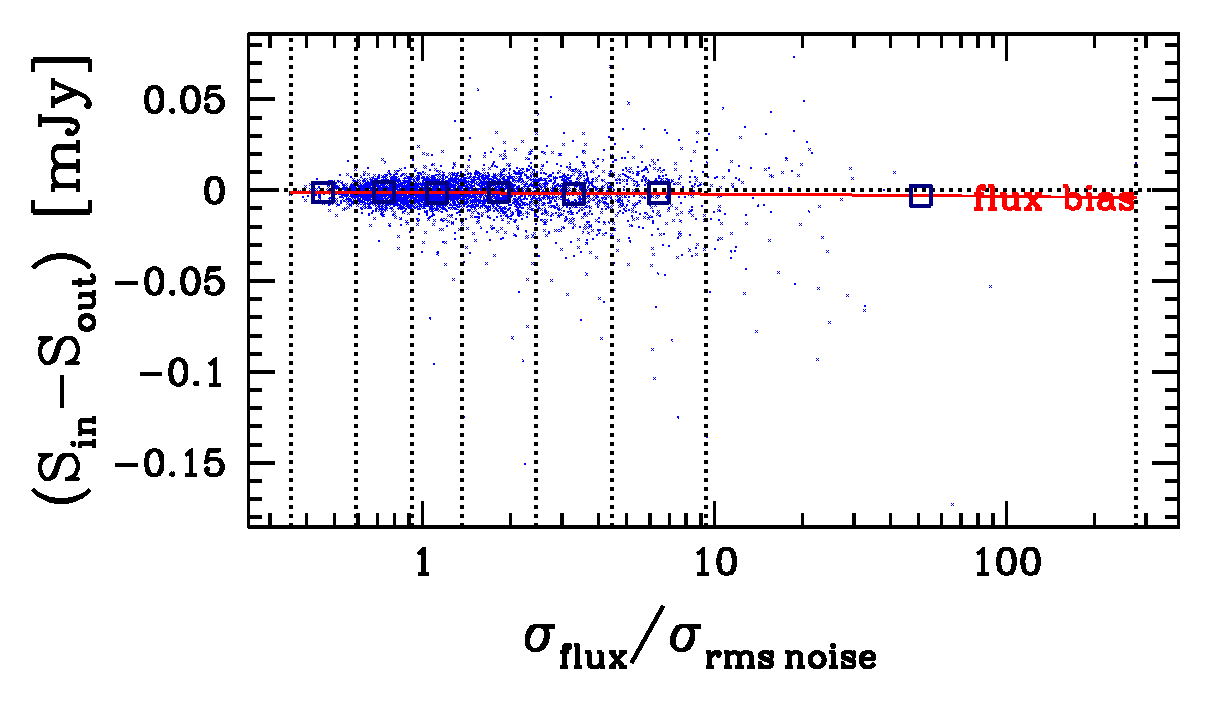
\includegraphics[width=0.8\textwidth]{galsim_24_fbias_1}
	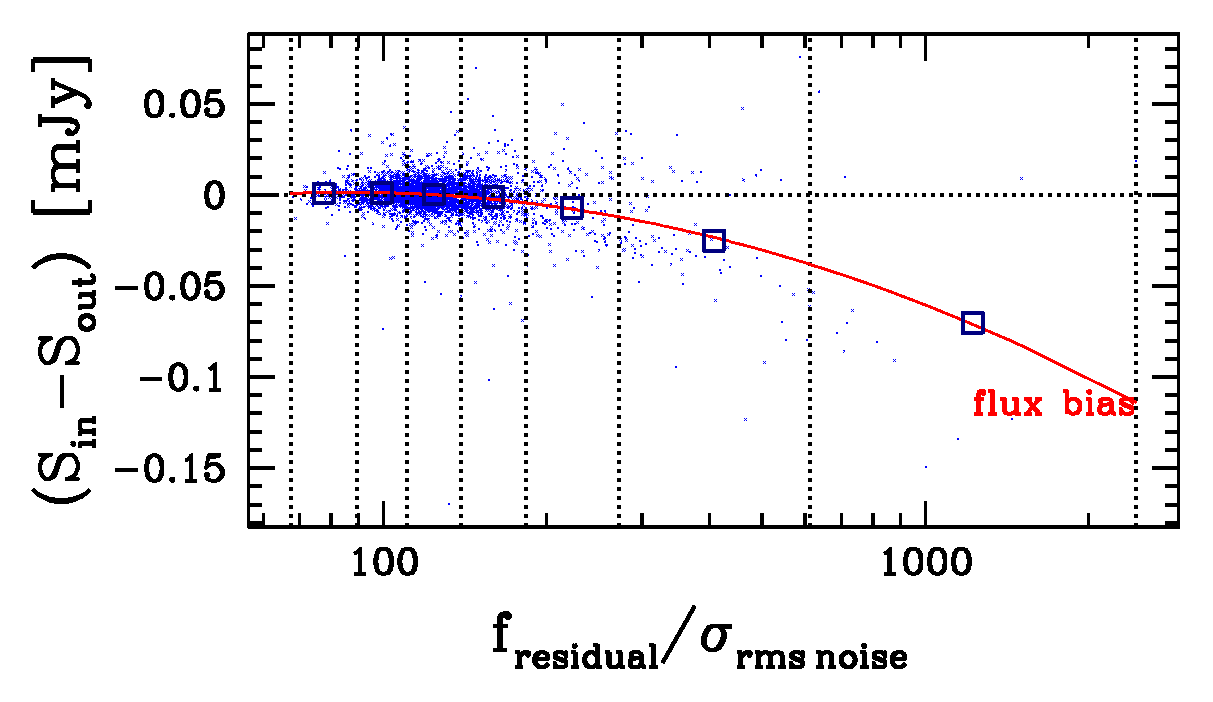
\includegraphics[width=0.8\textwidth]{galsim_24_fbias_2}
	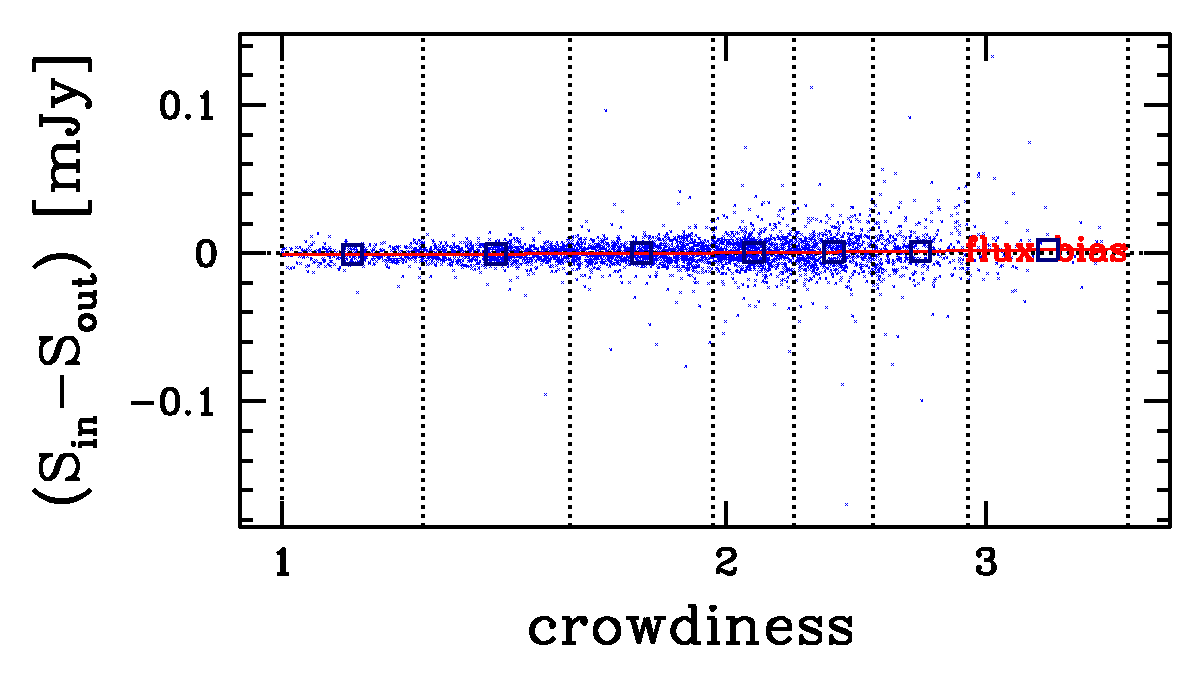
\includegraphics[width=0.8\textwidth]{galsim_24_fbias_3}
	\caption{Flux bias analysis from simulation.}
\end{figure}

\begin{figure}[H]
	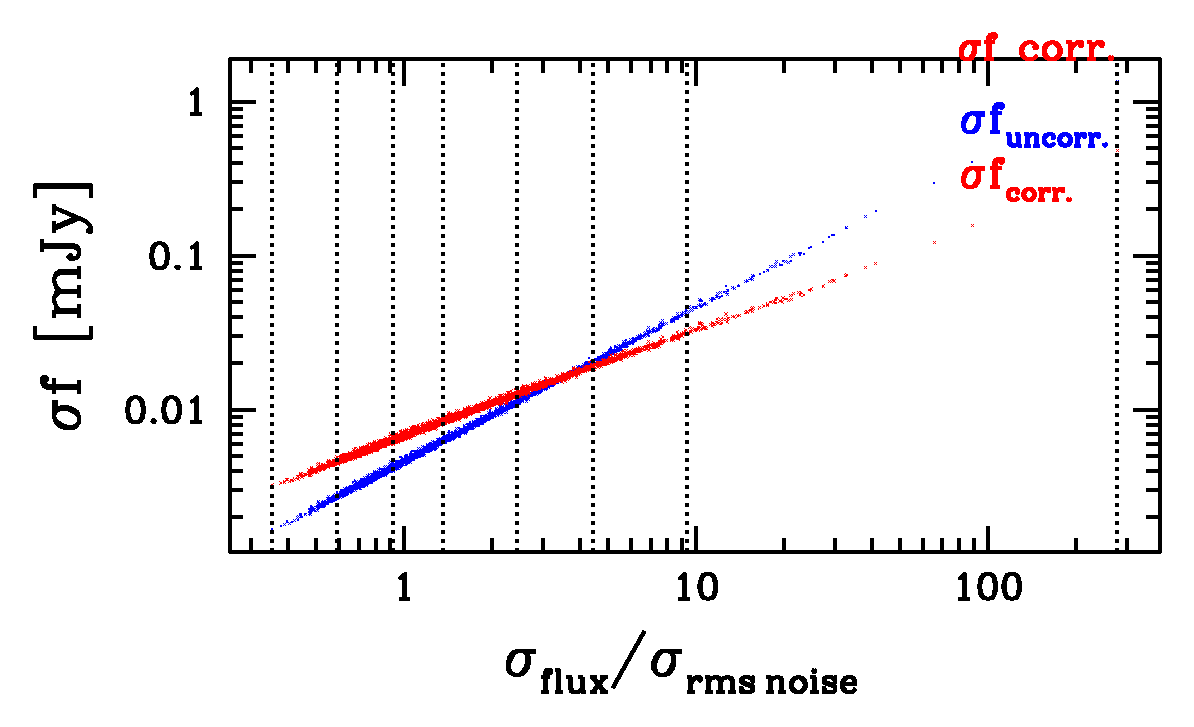
\includegraphics[width=0.8\textwidth]{galsim_24_dfcorr_1}
	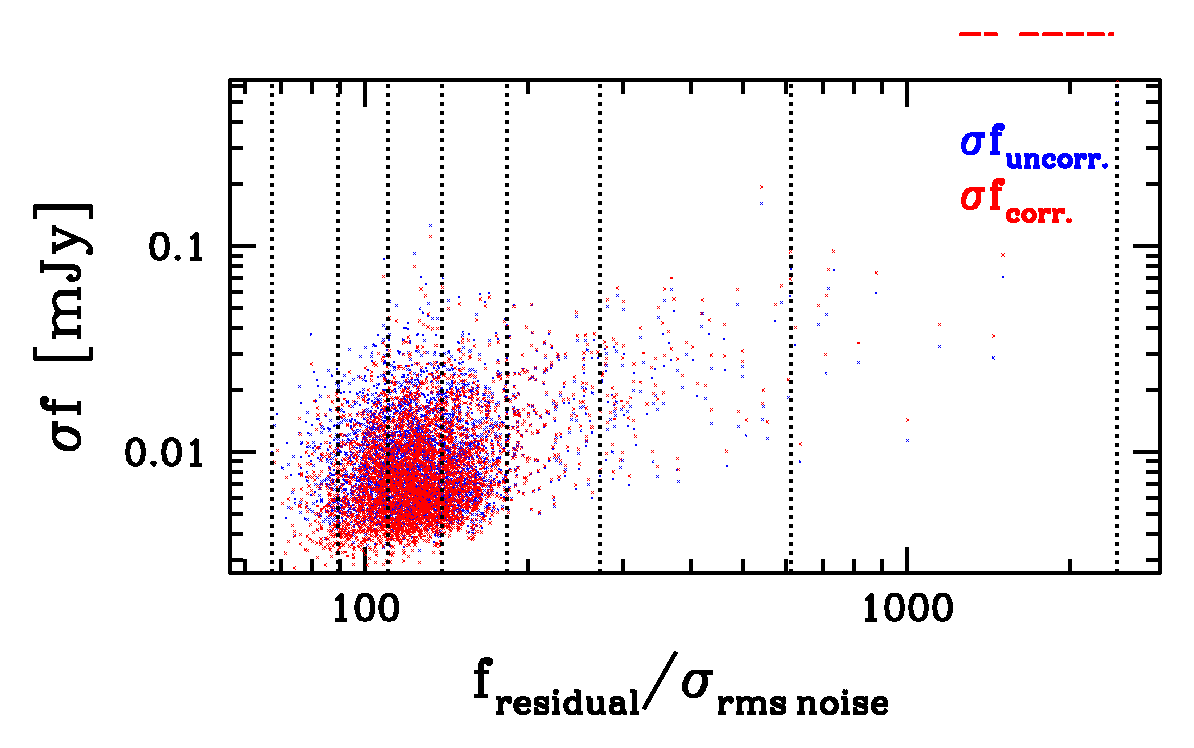
\includegraphics[width=0.8\textwidth]{galsim_24_dfcorr_2}
	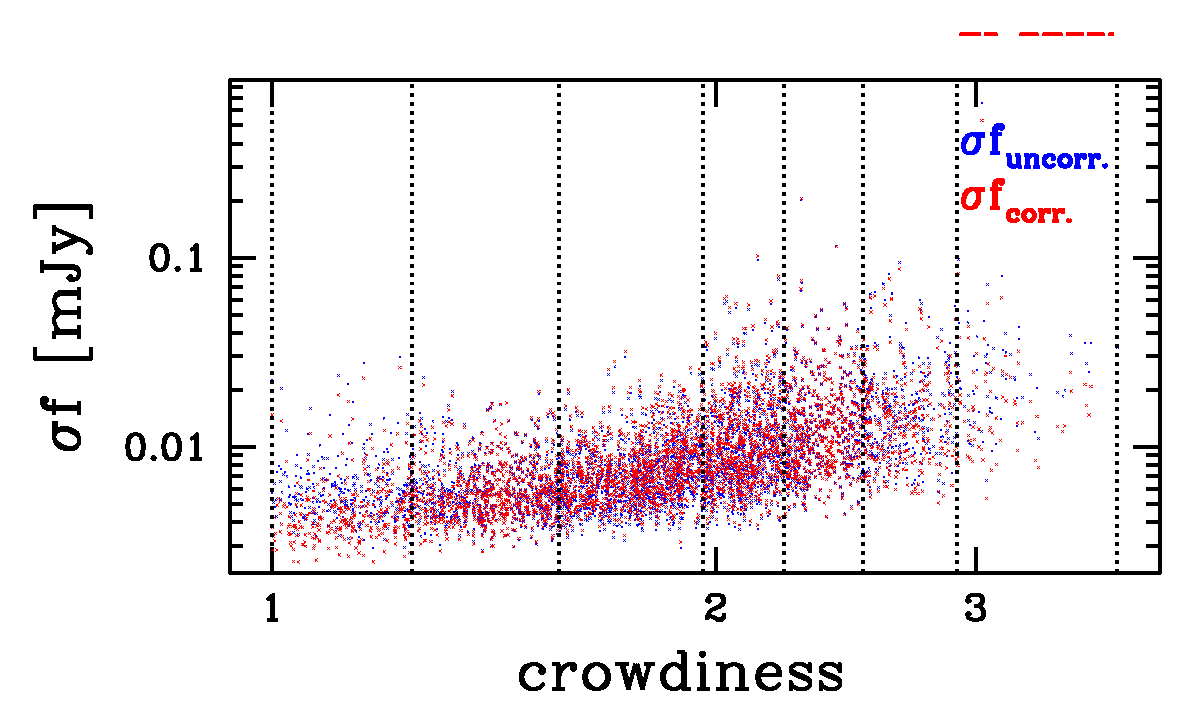
\includegraphics[width=0.8\textwidth]{galsim_24_dfcorr_3}
	\caption{Flux uncertainty analysis from simulation.}
\end{figure}

\begin{figure}[H]
	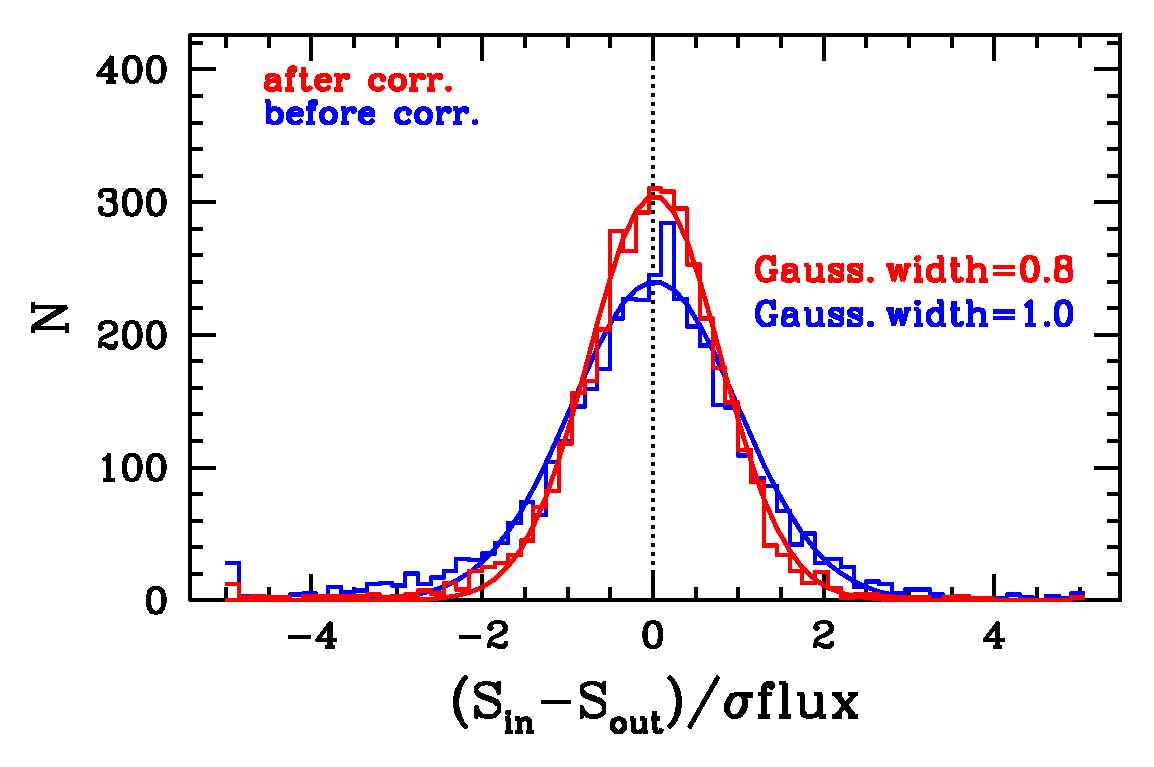
\includegraphics[width=0.8\textwidth]{galsim_24_hist_dfcorr_1}
	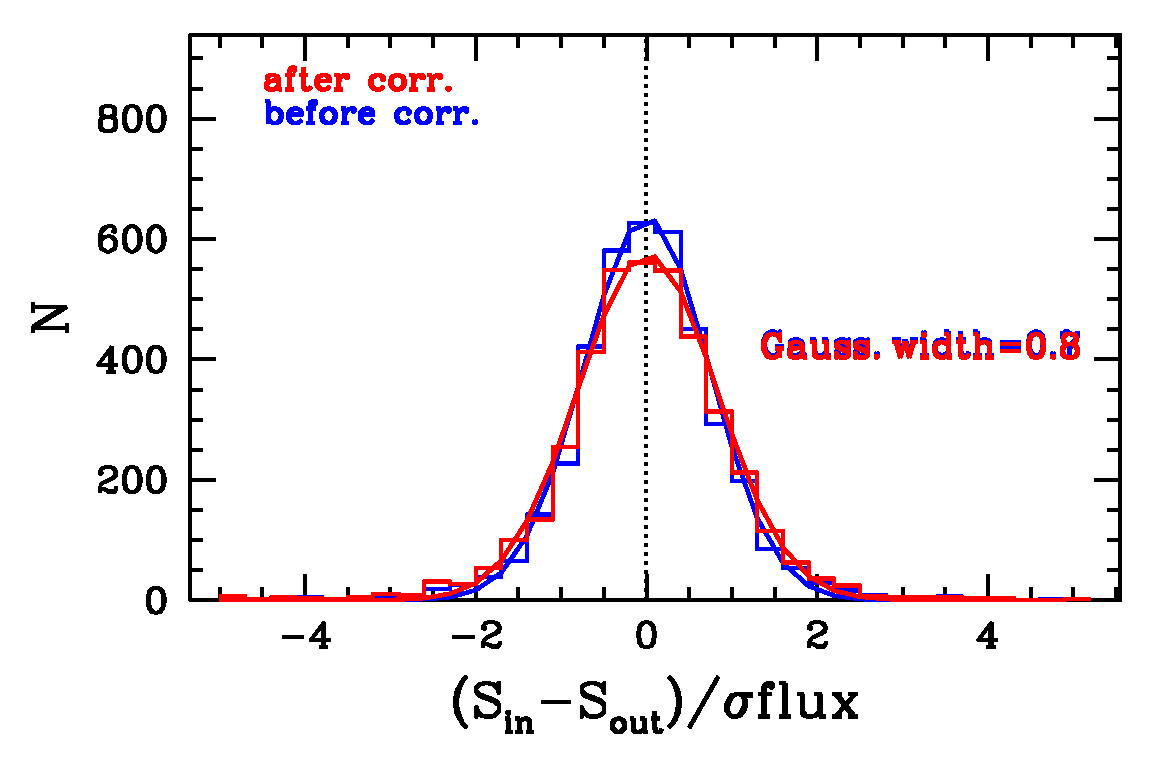
\includegraphics[width=0.8\textwidth]{galsim_24_hist_dfcorr_2}
	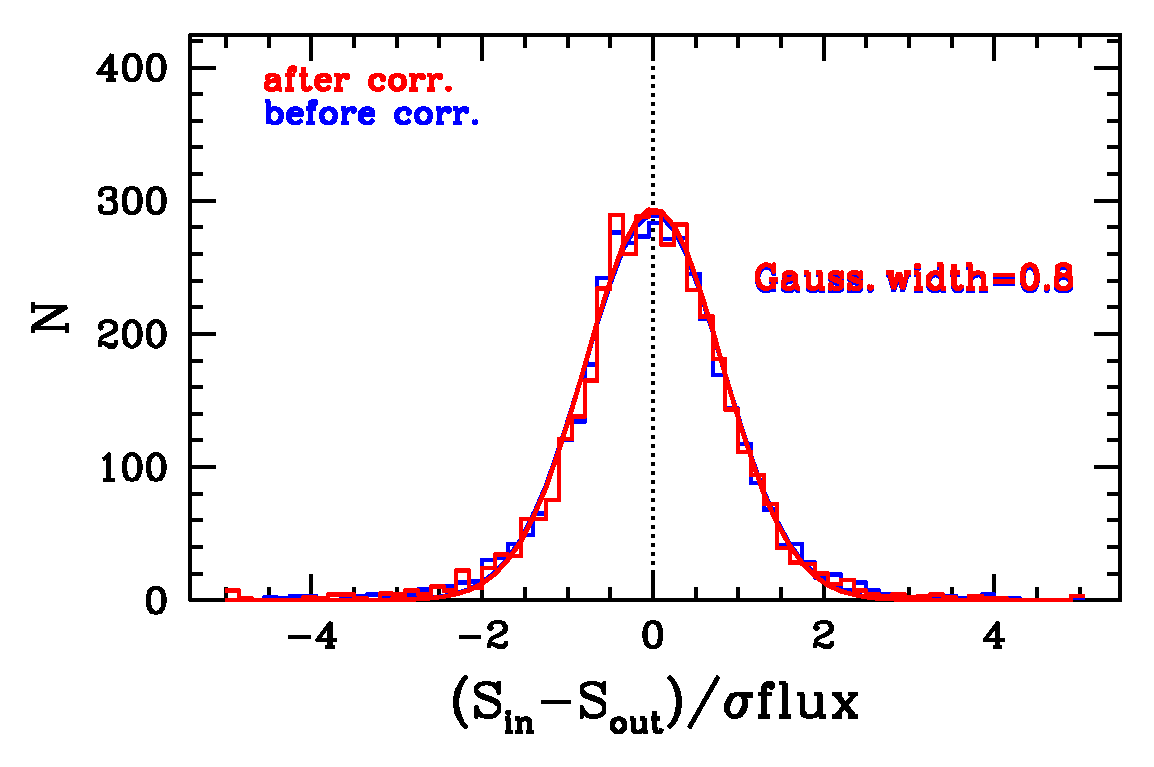
\includegraphics[width=0.8\textwidth]{galsim_24_hist_dfcorr_3}
	\caption{Statistical behavior of input minus output differences before and after correction.}
\end{figure}

%*************************************************************************************

\clearpage



%*************************************************************************************
\end{document}